\section{Introduction}

\begin{frame}{The Internet of Things (IoT)}
    \begin{columns}
        \begin{column}{0.58\textwidth}
            \small
            \textbf{What is IoT?}
            \begin{itemize}
                \item A network of everyday physical objects -- sensors, actuators, smart
                devices -- embedded with computing and connectivity.
                \item They \textbf{sense, exchange, and act} on data with little human
                intervention, reporting to gateways/cloud over an \textbf{open wireless channel}
                (often via multihop relays).
            \end{itemize}

            \vspace{0.15cm}
            \textbf{Why is authentication needed?}
            \begin{itemize}
                \item Authentication ensures that \textbf{only legitimate devices} participate in
                the network -- preventing \textbf{impersonation}, \textbf{unauthorized access}, and
                \textbf{replay attacks}, and enabling \textbf{secure session-key establishment}.
            \end{itemize}
        \end{column}
        \begin{column}{0.42\textwidth}
            \centering
            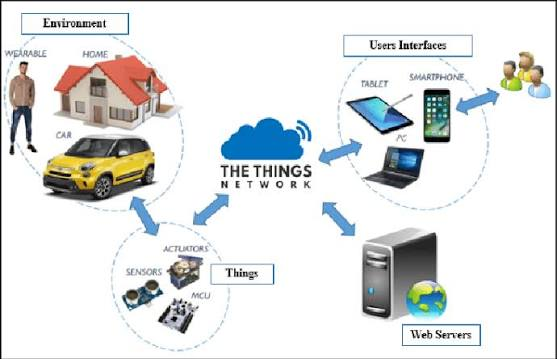
\includegraphics[width=0.88\columnwidth,height=0.42\textheight,keepaspectratio]{images.jpg}

            \vspace{0.4cm}
            \begin{block}{Core tension}
                \centering
                \textbf{Strong security} \quad vs. \quad \textbf{Low energy / CPU cost}\\[0.2cm]
                \footnotesize on devices that cannot afford heavy cryptography.
            \end{block}
        \end{column}
    \end{columns}
\end{frame}

\begin{frame}{Centralized vs.\ Distributed Authentication}
    \begin{block}{Centralized schemes}
        All authentication traffic is routed through a single gateway $\Rightarrow$
        \textbf{excessive relay load} on intermediate nodes in a multihop topology.
    \end{block}

    \begin{block}{Distributed schemes}
        Each parent authenticates its own children $\Rightarrow$ whichever node a burst of
        new devices joins under is \textbf{overloaded}, while other capable nodes stay \textbf{idle}.
        This is the \textbf{skewed-load} problem.
    \end{block}

    \vspace{0.2cm}
    \begin{alertblock}{DAuth -- base scheme~\cite{dauth}}
        A \textbf{decoupled} distributed scheme: the gateway pre-assigns \emph{any} capable node
        (parent \emph{or} non-parent) as the Authentication Server (AS), spreading the load evenly.
        Uses \textbf{PUF}-based secrets, a \textbf{hash-based accumulator}, and \textbf{XOR}-masked messages.
    \end{alertblock}
\end{frame}
